\documentclass[xcolor=dvipsnames,aspectratio=169]{beamer}

\usepackage{fontspec}
\defaultfontfeatures{Ligatures=TeX}
%\setsansfont{Liberation Sans}
\usepackage{polyglossia}
\setdefaultlanguage{german}

\usetheme{Berlin}
\usecolortheme[named=LimeGreen]{structure}
\usepackage{beamerthemesplit} % kam neu dazu
	
\usepackage{amsmath}
\usepackage{graphicx}
\graphicspath{{pictures/}}
\usepackage{amssymb}
\usepackage{amsfonts}
\usepackage{caption}
\usepackage{multimedia}
\usepackage{tikz}
\usepackage{listings}
\usepackage{acronym}
\usepackage{uhrzeit}
\usepackage{lmodern}
\usepackage{multicol}
\usepackage{csquotes}
\usepackage{pgfplots}

\definecolor{pblue}{rgb}{0.13,0.13,1}
\definecolor{pgreen}{rgb}{0,0.5,0}
\definecolor{pred}{rgb}{0.9,0,0}
\definecolor{pgrey}{rgb}{0.46,0.45,0.48}

\newcounter{countitems}
\newcounter{nextitemizecount}
\newcommand{\setupcountitems}{%
  \stepcounter{nextitemizecount}%
  \setcounter{countitems}{0}%
  \preto\item{\stepcounter{countitems}}%
}
\makeatletter
\newcommand{\computecountitems}{%
  \edef\@currentlabel{\number\c@countitems}%
  \label{countitems@\number\numexpr\value{nextitemizecount}-1\relax}%
}
\newcommand{\nextitemizecount}{%
  \getrefnumber{countitems@\number\c@nextitemizecount}%
}
\newcommand{\previtemizecount}{%
  \getrefnumber{countitems@\number\numexpr\value{nextitemizecount}-1\relax}%
}

\makeatother    
\newenvironment{AutoMultiColItemize}{%
\ifnumcomp{\nextitemizecount}{>}{3}{\begin{multicols}{2}}{}%
\setupcountitems\begin{itemize}}%
{\end{itemize}%
\unskip\computecountitems\ifnumcomp{\previtemizecount}{>}{3}{\end{multicols}}{}}

\lstset{
    escapeinside={(*}{*)}
}


\lstdefinelanguage{custom}
{
morekeywords={public, void},
sensitive=false,
morecomment=[l]{//},
morecomment=[s]{/*}{*/},
morestring=[b]",
}


\lstdefinestyle{BashInputStyle}{
  language=bash,
  showstringspaces=false,
  basicstyle=\small\sffamily,
  numbers=left,
  numberstyle=\tiny,
  numbersep=5pt,
  frame=trlb,
  columns=fullflexible,
  backgroundcolor=\color{gray!20},
  linewidth=0.9\linewidth,
  xleftmargin=0.1\linewidth
}

   \pgfplotsset{
    standard/.style={%Axis format configuration
        axis x line=middle,
        axis y line=middle,
        enlarge x limits=0.15,
        enlarge y limits=0.15,
        every axis x label/.style={at={(current axis.right of origin)},anchor=north west},
        every axis y label/.style={at={(current axis.above origin)},anchor=north east},
        every axis plot post/.style={mark options={fill=white}}
        }
    }
    

%Logo in the upper right just change if you know what you are doing^^
\addtobeamertemplate{frametitle}{}{%
\begin{tikzpicture}[remember picture,overlay]
\node[anchor=north east,yshift=2pt] at (current page.north east) {
\includegraphics[height=1.8cm]{htw}};
\end{tikzpicture}}

\begin{document}
\bibliographystyle{alpha}
\title{Technische und logische Grundlagen der Informatik\\Wintersemester 2021/22}
\subtitle{Signale im Zeit und Frequenzbereich\\

\href{mailto:Benjamin.Troester@HTW-Berlin.de}{Benjamin.Troester@HTW-Berlin.de}\\
		PGP: ADE1 3997 3D5D B25D 3F8F 0A51 A03A 3A24 978D D673 }

\author{Benjamin Tröster}

\date{}

\begin{frame}
\titlepage
\end{frame}

\section*{Road-Map}
\begin{frame}
\frametitle{Road-Map}
\begin{multicols}{2}
  \tableofcontents
\end{multicols}
\end{frame}

\section{Signal}
\begin{frame}{Signal}
\begin{itemize}
\begin{definition}[Signal]
  		Informationstragende, physikalische Größe, die sich über der Zeit, über dem Ort oder über einer anderen Variablen ändert.
\end{definition}
	\item Mathematisch: Funktion einer oder mehrerer Variablen, z.B. $ y(t) = m\cdot x + n, r^2 = (x - x_0)^2 + (y - y_0)^2 + (z - z_0)^2$ 
	\item Beispiele: Temperatur über der Zeit $x(t)$, Helligkeit eines Bildes $l(x,y)$, Schalldruck $\rho(x,y,z,t)$ etc.
	\item Unterscheidung in deterministische (periodische) oder stochastische Signale
\end{itemize}
\end{frame}


\subsection{Illustratives Beispiel}

\begin{frame}
	\begin{itemize}
		\item Zeitkontinuierlich Luftdruckschwankungen:\\Musik und Sprache
	\end{itemize}
	\begin{figure}
	\centering
	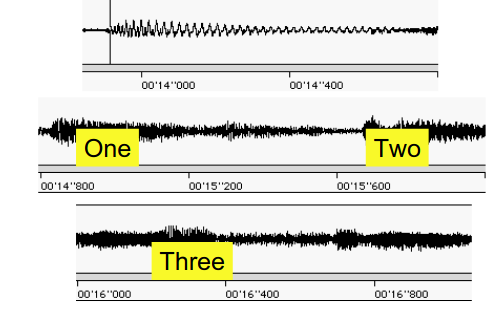
\includegraphics[scale=0.5]{audio}
	\end{figure}
\end{frame}


\subsection{Analoge/Digitale Signale}
\begin{frame}{Analoge/Digitale Signale}
\begin{itemize}
	\item Analoge Signale sind wert- \& zeitkontinuierlich
	\begin{itemize}
		\item Werte kontinuierlich (stetig)
		\item I.A. alle natürlichen physikalischen Signale \& Prozesse
	\end{itemize}
	\item Digitale Signale sind wert- \& zeitdiskret
	\begin{itemize}
		\item Diskrete Werte
		\item Variablen-Diskretisierung (Abtastung, führt zu diskreten Signalen)
		\item Amplituden- bzw. Wert-Diskretisierung (Quantisierung)
	\end{itemize}	
\end{itemize}
\end{frame}

\section{Digital vs. Analog}

\begin{frame}{Digital vs. Analog}
\begin{columns}[T] % align columns
\begin{column}{.48\textwidth}
\begin{itemize}
\vspace{-1cm}
		\item Analog:\\
		\begin{tikzpicture}[scale=.85]
  \begin{axis}%
    [grid=both,
     minor tick num=4,
     grid style={line width=.1pt, draw=gray!10},
     major grid style={line width=.2pt,draw=gray!50},
     axis lines=middle,
     enlargelimits={abs=0.2},
    ]
    \addplot[domain=-0:3,samples=50,smooth,red] {sin(deg(pi*x))};
  \end{axis}
\end{tikzpicture}
	\end{itemize} 
\end{column}%
\hfill%
\begin{column}{.48\textwidth}
\begin{itemize}
\vspace{-1cm}
	\item Digital:\\
\begin{tikzpicture}[scale=.85]
            \begin{axis}[%
            grid=both,
     minor tick num=4,
     grid style={line width=.1pt, draw=gray!10},
     major grid style={line width=.2pt,draw=gray!50},
     axis lines=middle,
     enlargelimits={abs=0.2},
                standard,
                domain = 0:3,
                samples = 5]
                \addplot+[ycomb,black,thick] {sin(deg(pi*x))};
            \end{axis}
        \end{tikzpicture}
        \end{itemize}
\end{column}%
\end{columns}
\end{frame}

\begin{frame}{Digital vs. Analog}
\begin{columns}[T] % align columns
\begin{column}{.48\textwidth}
\begin{itemize}
\vspace{-1cm}
		\item Analog:\\
		\begin{tikzpicture}[scale=.85]
  \begin{axis}%
    [grid=both,
     minor tick num=4,
     grid style={line width=.1pt, draw=gray!10},
     major grid style={line width=.2pt,draw=gray!50},
     axis lines=middle,
     enlargelimits={abs=0.2},
    ]
    \addplot[domain=-0:3,samples=50,smooth,red] {sin(deg(pi*x))};
  \end{axis}
\end{tikzpicture}
	\end{itemize} 
\end{column}%
\hfill%
\begin{column}{.48\textwidth}
\begin{itemize}
\vspace{-1cm}
	\item Digital:\\
\begin{tikzpicture}[scale=.85]
            \begin{axis}[%
            grid=both,
     minor tick num=4,
     grid style={line width=.1pt, draw=gray!10},
     major grid style={line width=.2pt,draw=gray!50},
     axis lines=middle,
     enlargelimits={abs=0.2},
                standard,
                domain = 0:3,
                samples = 16]
                \addplot+[ycomb,black,thick] {sin(deg(pi*x))};
            \end{axis}
        \end{tikzpicture}
        \end{itemize}
\end{column}%
\end{columns}
\end{frame}

\begin{frame}{Digital vs. Analog}
\begin{columns}[T] % align columns
\begin{column}{.48\textwidth}
\vspace{-1cm}
\begin{itemize}
		\item Analog:\\
		\begin{tikzpicture}[scale=.85]
  \begin{axis}%
    [grid=both,
     minor tick num=4,
     grid style={line width=.1pt, draw=gray!10},
     major grid style={line width=.2pt,draw=gray!50},
     axis lines=middle,
     enlargelimits={abs=0.2},
    ]
    \addplot[domain=-0:3,samples=50,smooth,red] {sin(deg(pi*x))};
  \end{axis}
\end{tikzpicture}
	\end{itemize} 
\end{column}%
\hfill%
\begin{column}{.48\textwidth}
\vspace{-1cm}
\begin{itemize}
	\item Digital:\\
\begin{tikzpicture}[scale=.85]
            \begin{axis}[%
            grid=both,
     minor tick num=4,
     grid style={line width=.1pt, draw=gray!10},
     major grid style={line width=.2pt,draw=gray!50},
     axis lines=middle,
     enlargelimits={abs=0.2},
                standard,
                domain = 0:3,
                samples = 32]
                \addplot+[ycomb,black,thick] {sin(deg(pi*x))};
            \end{axis}
        \end{tikzpicture}
        \end{itemize}
\end{column}%
\end{columns}
\end{frame}

\begin{frame}{Bits}
\begin{itemize}
	\item Digitale Signale: diskret
	\item Einfachste Diskretisierung: binäres Alphabet $\mathbb{B} = \{0,1\}$
	\begin{itemize}
		\item Bit Kunstwort von Binary Digit
	\end{itemize}
	\item Darstellung in \enquote{An, Aus; Strom, kein Strom; Licht, kein Licht}
\end{itemize}
\end{frame}

\section{Anwendungsbeispiel: Netzwerke}
\begin{frame}{Anwendungsbeispiel: Netzwerke}
\begin{columns}[T] % align columns
\begin{column}{.54\textwidth}
\begin{itemize}
	\item Daten werden konvertiert über einen Kanal gesendet
	\item Übertragungskanal: Access Point + Übertragungsmedium des physikalischen Mediums
	\begin{itemize}
		\item Kupferkabel, Glasfaser, Radiowelle, etc.
	\end{itemize}
\end{itemize}
\end{column}%
\hfill%
\begin{column}{.48\textwidth}
\begin{figure}
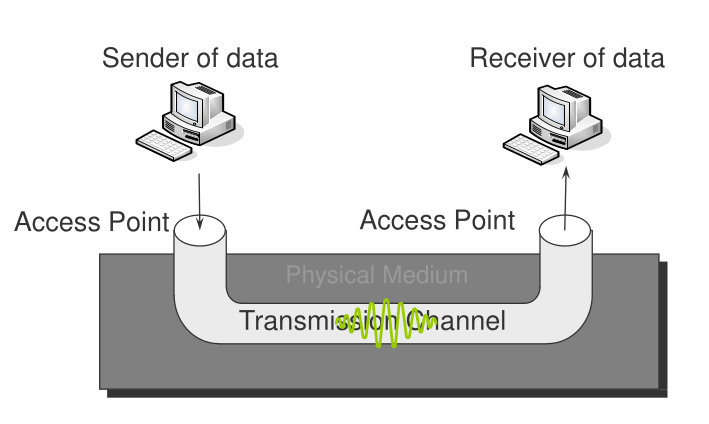
\includegraphics[scale=0.3]{rxtx}
\end{figure}
\end{column}%
\end{columns}
\end{frame}

\begin{frame}{Computers deal with digital signals}
\begin{columns}[T] % align columns
\begin{column}{.48\textwidth}
\begin{itemize}
	\item Quantisierung -- The need to convert
	\begin{itemize}
		\item Computer arbeiten ausschließlich mit digitalen Daten $to$ diskreten Signalen
		\item Physikalische Medien sind aber immer analoge $to$ kontinuierliche Signale
		\item Also muss eine Konvertierung von digital zu analog erfolgen (vice versa)
	\end{itemize}
\end{itemize}
\end{column}%
\hfill%
\begin{column}{.48\textwidth}
\begin{figure}
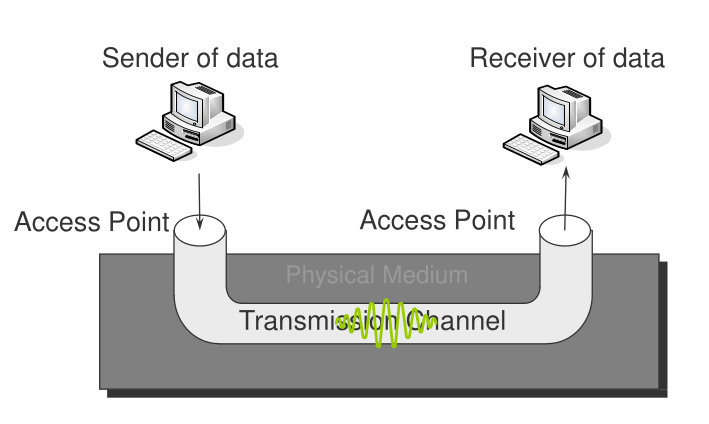
\includegraphics[scale=0.3]{rxtx}
\end{figure}
\end{column}%
\end{columns}
\end{frame}

\begin{frame}{Computers deal with digital signals}
\begin{columns}[T] % align columns
\begin{column}{.48\textwidth}
\begin{itemize}
	\item Abstastung -- The need to measure
	\begin{itemize}
		\item Computer haben nur eine diskrete Auflösung der Zeit (Quarz)
		\item Zustand des physikalische Mediums variiert stetig
	\end{itemize}
\end{itemize}
\end{column}%
\hfill%
\begin{column}{.48\textwidth}
\begin{figure}
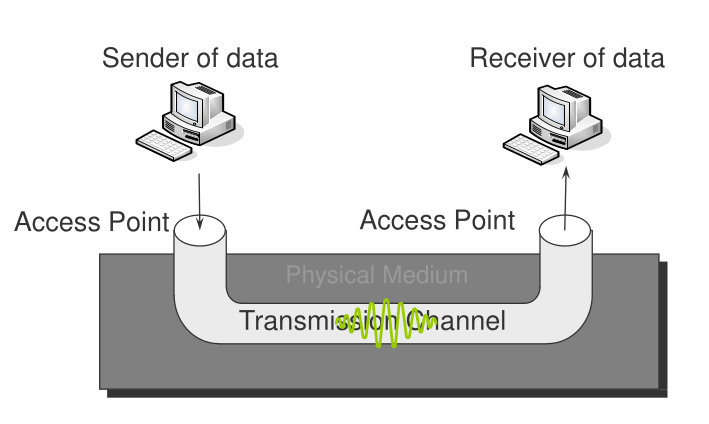
\includegraphics[scale=0.3]{rxtx}
\end{figure}
\end{column}%
\end{columns}
\end{frame}

\subsection{Signalverarbeitungsarchitekturen}
\begin{frame}{Signalverarbeitungsarchitekturen}
\begin{itemize}
	\item Analoge Signalverarbeitung:\\
	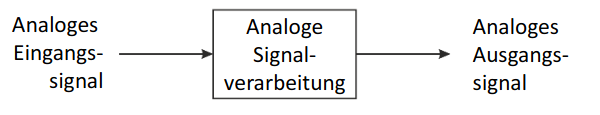
\includegraphics[scale=0.35]{analog}
	\item Digitale Signalverarbeitung:\\
	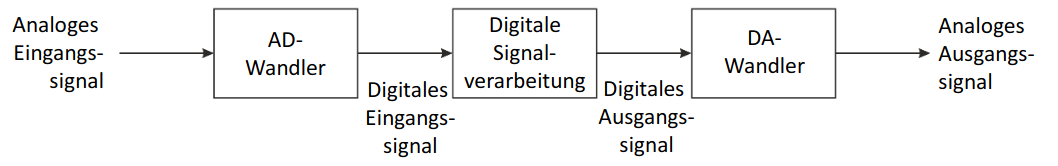
\includegraphics[scale=0.35]{ds}
\end{itemize}
\end{frame}

\begin{frame}{Analog $\to$ Digital}
\vspace{-.74cm}
	\begin{figure}
	\centering
	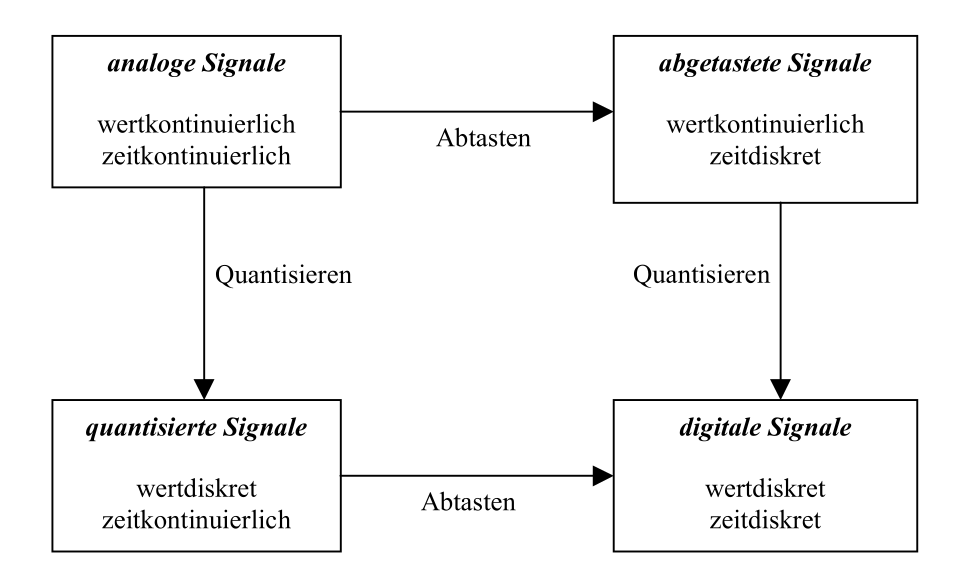
\includegraphics[scale=0.28]{adda}
	\end{figure}
\end{frame}

\section{Grundlegende Signalverarbeitung: Deterministische Signale}
\begin{frame}{Grundlegende Signalverarbeitung: Deterministische Signale}
\begin{columns}[T] % align columns
\begin{column}{.6\textwidth}
\begin{itemize}
	\item Periodische Signale $\to$ deterministisch, Periode gibt fixen Bereich vor
	\item Parameter periodische Signale:
	\begin{itemize}
		\item Periode $T$
		\item Frequenz $f=\frac{1}{T}$, 
		\item Amplitude $S(t)$
		\item Phase $\varphi$
	\end{itemize}
	\item Beispiele:
	\begin{itemize}
		\item Sinus: Periode $2\pi$
		\item Phase shift $\varphi$ ($\sin \to \cos: \varphi= \frac{3}{2} \pi$)
	\end{itemize}
\end{itemize}
\end{column}%
\hfill%
\begin{column}{.4\textwidth}
\vspace*{-.75cm}
\begin{figure}
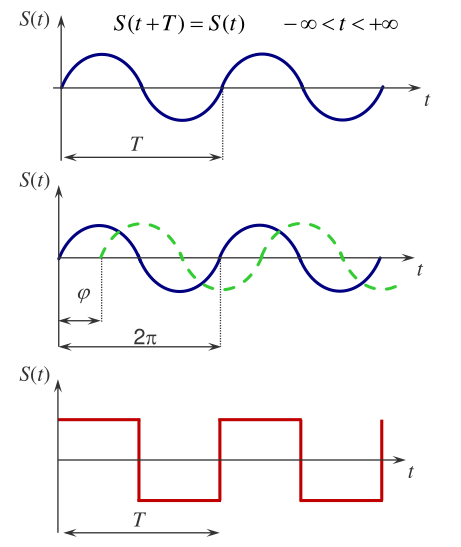
\includegraphics[scale=0.3]{sigproc}
\end{figure}
\end{column}%
\end{columns}
\end{frame}

\begin{frame}{Komposition periodischer Signale}
\begin{columns}[T] % align columns
\begin{column}{.6\textwidth}
\begin{itemize}
	\item Periodische Funktionen als Kompositionen
	\begin{itemize}
		\item Beispiel: $s(t) = \sin(2\pi f t) + \frac{1}{3} \sin(2\pi (3f) t)$
	\end{itemize}
	\item Signal: Sin mit Frequenz $f$ und $3f$
	\begin{figure}
	\centering
	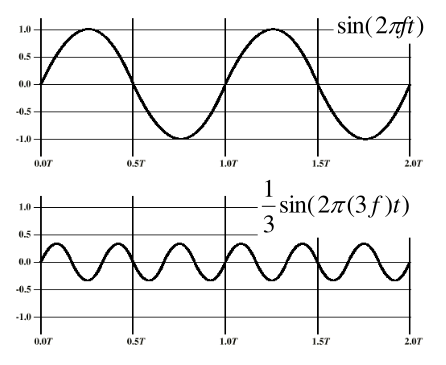
\includegraphics[scale=0.3]{sin}
	\end{figure}
\end{itemize}
\end{column}%
\hfill%
\begin{column}{.4\textwidth}
\vspace*{.75cm}
\begin{figure}
\centering
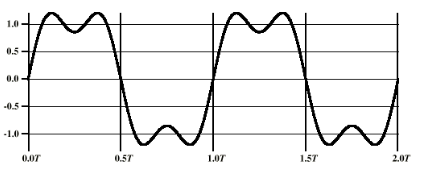
\includegraphics[scale=0.4]{comp}
\end{figure}
\end{column}%
\end{columns}
\end{frame}

\section{Fourier-Reihen}
\begin{frame}{Einschub Fourier-Reihen}
\begin{itemize}
	\item Jede periodische Funktion kann als Summe von Sinus- und Kosinusfunktionen dargestellt werden $\Leftarrow$ Fourier-Reihe
	\item Reihenentwicklung: Darstellung (komplizierten) Funktion durch die Summe (einfachen) Ersatzfunktionen
	\begin{itemize}
		\item Lineare mathematische Umformungen (Addition, Differentiation, Integration usw.) als Ersatzfunktionen statt Originalfunktion
		\item Reihendarstellung: Approximation, bei unendlich vielen Reihengliedern exakt (sofern Konvergent)
	\end{itemize}
	\item Stetiges periodisches Signal $x(t)$ kann durch Fourier-Reihe approximiert werden
	\item Wie viele Reihenglieder und somit Koeffizienten notwendig sind, hängt von den Eigenschaften von $x(t)$
\end{itemize}
\end{frame}

\section{Bit-Rate des Übertragungskanals}
\begin{frame}{Bit-Rate des Übertragungskanals}
\begin{columns}[T] % align columns
\begin{column}{.6\textwidth}
\begin{itemize}
	\item Beispiel: Rechteckschwingung 
	\begin{itemize}
		\item Positiver Puls 1-Bit
		\item Negativer Puls 0-Bit
		\item Dauer des Pulses $\frac{1}{2}f$
		\item Datenrate ist $2f$ Bits pro Sekunde
	\end{itemize}
	\item Bandbreite ist physikalisch begrenzt (Eigenschaft des Mediums)
	\begin{itemize}
		\item Berechnung: $\delta = f_{max} - f_{min}$
	\end{itemize}
\end{itemize}
\end{column}%
\hfill%
\begin{column}{.4\textwidth}
\vspace*{-.7cm}
\begin{figure}
\centering
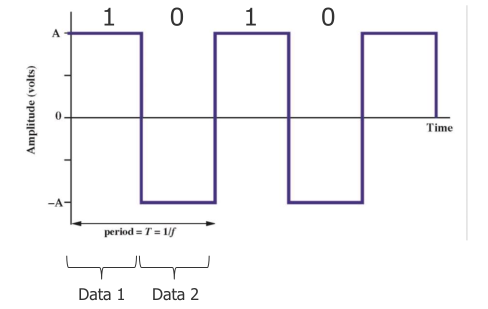
\includegraphics[scale=0.25]{square}
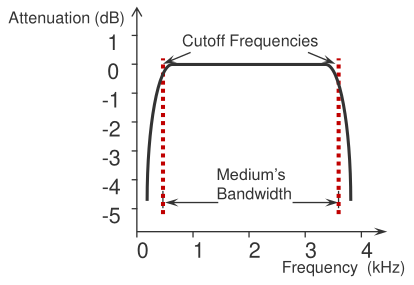
\includegraphics[scale=0.25]{bw}
\end{figure}
\end{column}%
\end{columns}
\end{frame}

\begin{frame}{Bit-Rate vs. Bandbreite: Signalfrequenz}
\begin{columns}[T] % align columns
\begin{column}{.6\textwidth}
\vspace*{-.7cm}
\begin{itemize}
	\item Ziel: Komposition der Rechteckschwingung durch periodische Funktion
	\item Signal besteht aus $f, 3f$ und $5f$
	\begin{itemize}
		\item $\sin(2\pi f t) + \frac{1}{3} sin(2 \pi 3 f t) + \frac{1}{5} sin(2 \pi 5 f t)$
	\end{itemize}
	\item Signal besteht aus $f, 3f, 5f$ und $7f$
	\begin{itemize}
		\item $\sin(2\pi f t) + \frac{1}{3} sin(2 \pi 3 f t) + \frac{1}{5} sin(2 \pi 5 f t) + \frac{1}{7} sin(2 \pi 7 f t)$
	\end{itemize}
	\item Rechteckschwingung:
	$$ s(t) = A \cdot \frac{4}{\pi} \cdot \sum_{k=1, k \text{ ungearde}}^\infty \frac{1}{k} \sin(2 \pi k f t) $$
\end{itemize}
\end{column}%
\hfill%
\begin{column}{.4\textwidth}
\vspace*{-.7cm}
\begin{figure}
\centering
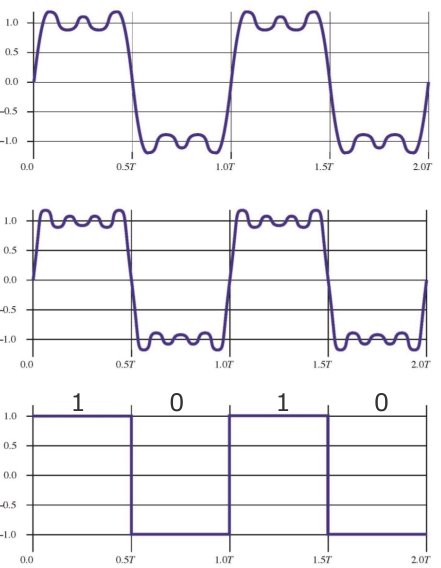
\includegraphics[scale=0.25]{sf}
\end{figure}
\end{column}%
\end{columns}
\end{frame}

\begin{frame}{Bit-Rate vs. Bandbreite: Medium limiting harmonics}
\begin{figure}
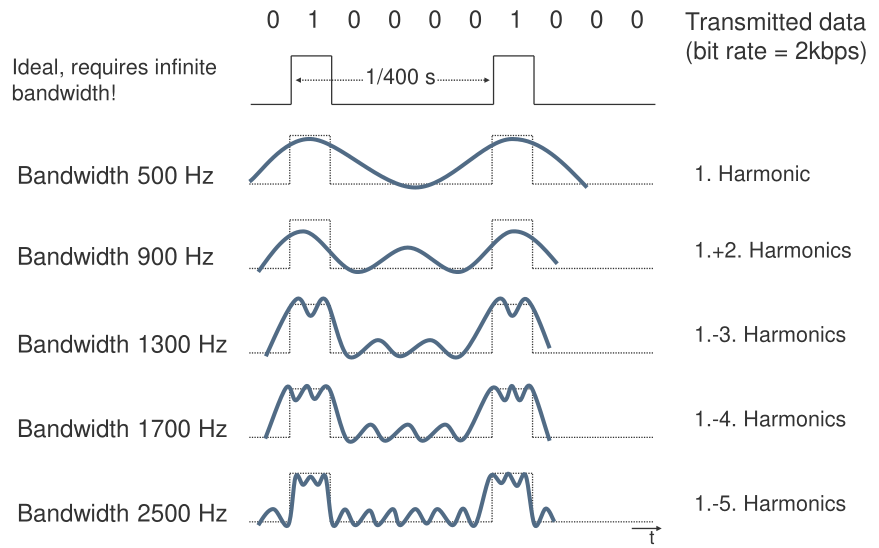
\includegraphics[scale=0.25]{harmonics}
\end{figure}
\end{frame}

\begin{frame}{Bit-Rate vs. Bandbreite: Numerisches Beispiel}
\begin{columns}[T] % align columns
\begin{column}{.6\textwidth}
\vspace*{-.7cm}
\begin{itemize}
	\item Beispiel Frequenz: $f = 1 MHz$
	\begin{itemize}
		\item Bandbreite des Signals: $s(t) = 5 \cdot 10^6 Hz) - (1 \cdot 10^6 Hz) = 4 MHz$
		\item Periode: $T = \frac{1}{T} = \frac{1}{10^6}s = 10^{-6}s = 1 \mu s$
		\item 1 Bit alle $0.5 \mu s$
		\item Datenrate: $r = 2 Bit \cdot 10^6 Hz = 2 \frac{MBit}{s}$
	\end{itemize}
	\item Beispiel: $f = 2 MHz$?
\end{itemize}
\end{column}%
\hfill%
\begin{column}{.4\textwidth}
\vspace*{-.7cm}
\begin{figure}
\centering
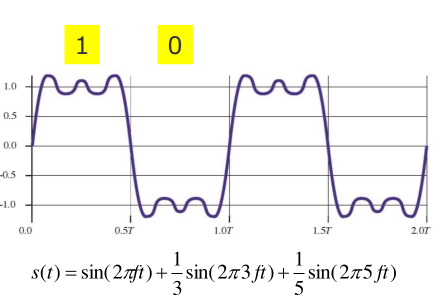
\includegraphics[scale=0.25]{bsp2}
\end{figure}
\end{column}%
\end{columns}
\end{frame}

\begin{frame}{Bit-Rate vs. Bandbreite: Multilevel Digital Signals}
\begin{itemize}
	\item Binäres Signal: Signal mit zwei Werten
	\item Multilevel digital Signal:
	\begin{itemize}
		\item Digitales Signal mit mehr als nur zwei Werten, DIBIT = zwei Bit pro Wert (quartär Signal)
		\item Anzahl der diskreten Werte eines Signals können wie folgt beschrieben werden:
		\begin{itemize}
			\item $n=2$ binary (binär)
			\item $n=3$ ternary (trinär)
			\item $n=4$ quaternary (quartär)
			\item ...
			\item $n=8$ octonary
			\item $n = 10$ denary
		\end{itemize}
	\end{itemize}
\end{itemize}
\end{frame}

\begin{frame}{Bit-Rate vs. Bandbreite: Multilevel Digital Signals}
\vspace*{-.7cm}
\begin{figure}
\centering
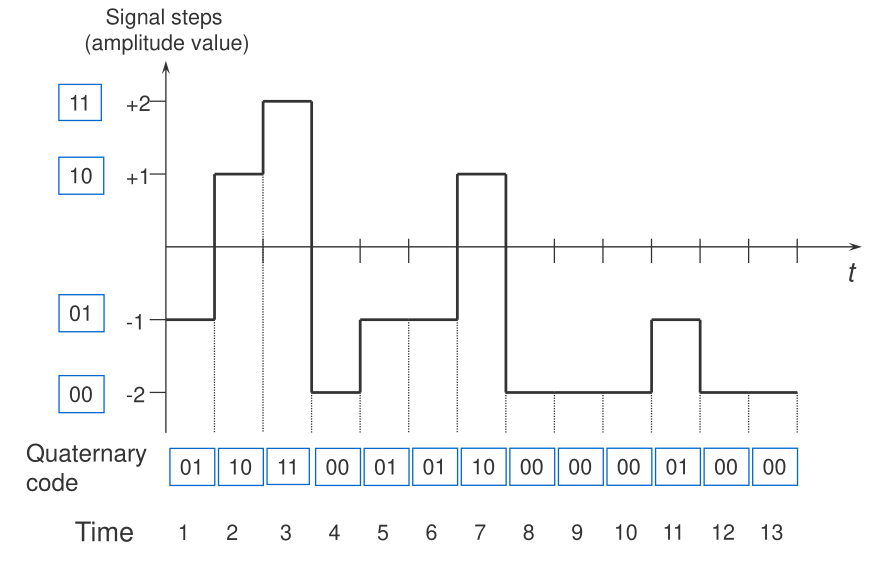
\includegraphics[scale=0.3]{bsp3}
\end{figure}
\end{frame}

\begin{frame}{Bit-Rate vs. Bandbreite: Datenrate}
Symbolrate = Anz. der physikalischen Ereignisse pro Zeiteinheit auf dem Medium\\
Einheit: Symbole/s = Baud (bd)

\begin{figure}
\centering
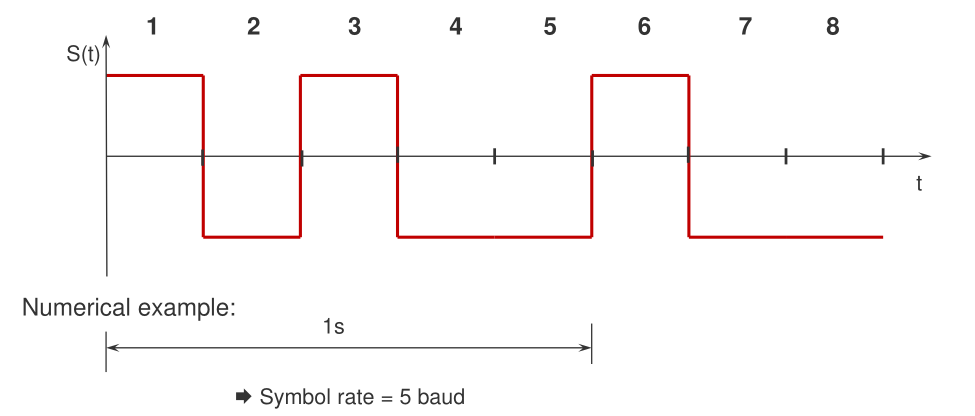
\includegraphics[scale=0.25]{bd}
\end{figure}
\end{frame}

\begin{frame}{Bit-Rate vs. Bandbreite: Datenrate}
\begin{itemize}
	\item Datenrate = Anzahl der dekodierten Bits der Symbolrate pro Zeiteinheit\\
Einheit: Bits/s (bps)
	\item Binäre Signale mit Frequenz $v$: Data rate $=v$\\
	Jedes Signal dekodiert 1 Bit
	\item Multilevel-Signale -- $n$ mögliche Werte: Data rate $= v \cdot \log_2(n)$
	\item Beispiel:
	\begin{itemize}
		\item DIBIT $\Leftarrow$ 1 baud = 2 bps (quaternary signal)
		\item TRIBIT $\Leftarrow$ 1 baud = 3 bps (octonary signal)
	\end{itemize}
\end{itemize}
\end{frame}

\begin{frame}{Bits \& Bytes}
\begin{figure}
	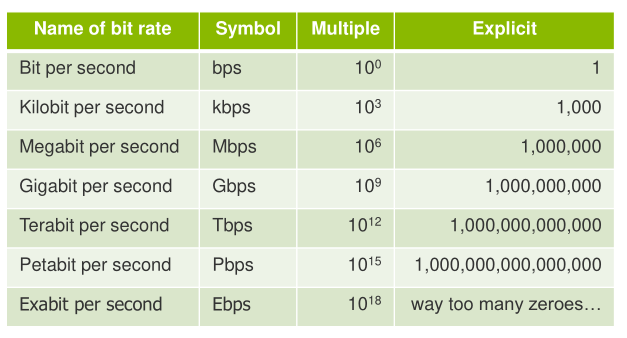
\includegraphics[scale=.4]{tab1}
\end{figure}
\end{frame}

\end{document}